\section{Case Study}

\label{sec_caseStudy}
In this section, we give \emph{(i)} a description of the ensemble (made publicly
available \cite{data})
% data
representing the Kelvin Helmholtz Instabilities (KHI) computed on 
%the CEA 
our institution's
facilities.
% which has 
% been 
% .
Next, we state \emph{(ii)} the challenges in understanding
such phenomena and we
% edict
provide
\emph{(iii)} theoretical hypothesis that our
experimental protocols have to verify.   

\begin{figure}
 \centering
 \vspace{-1ex}
 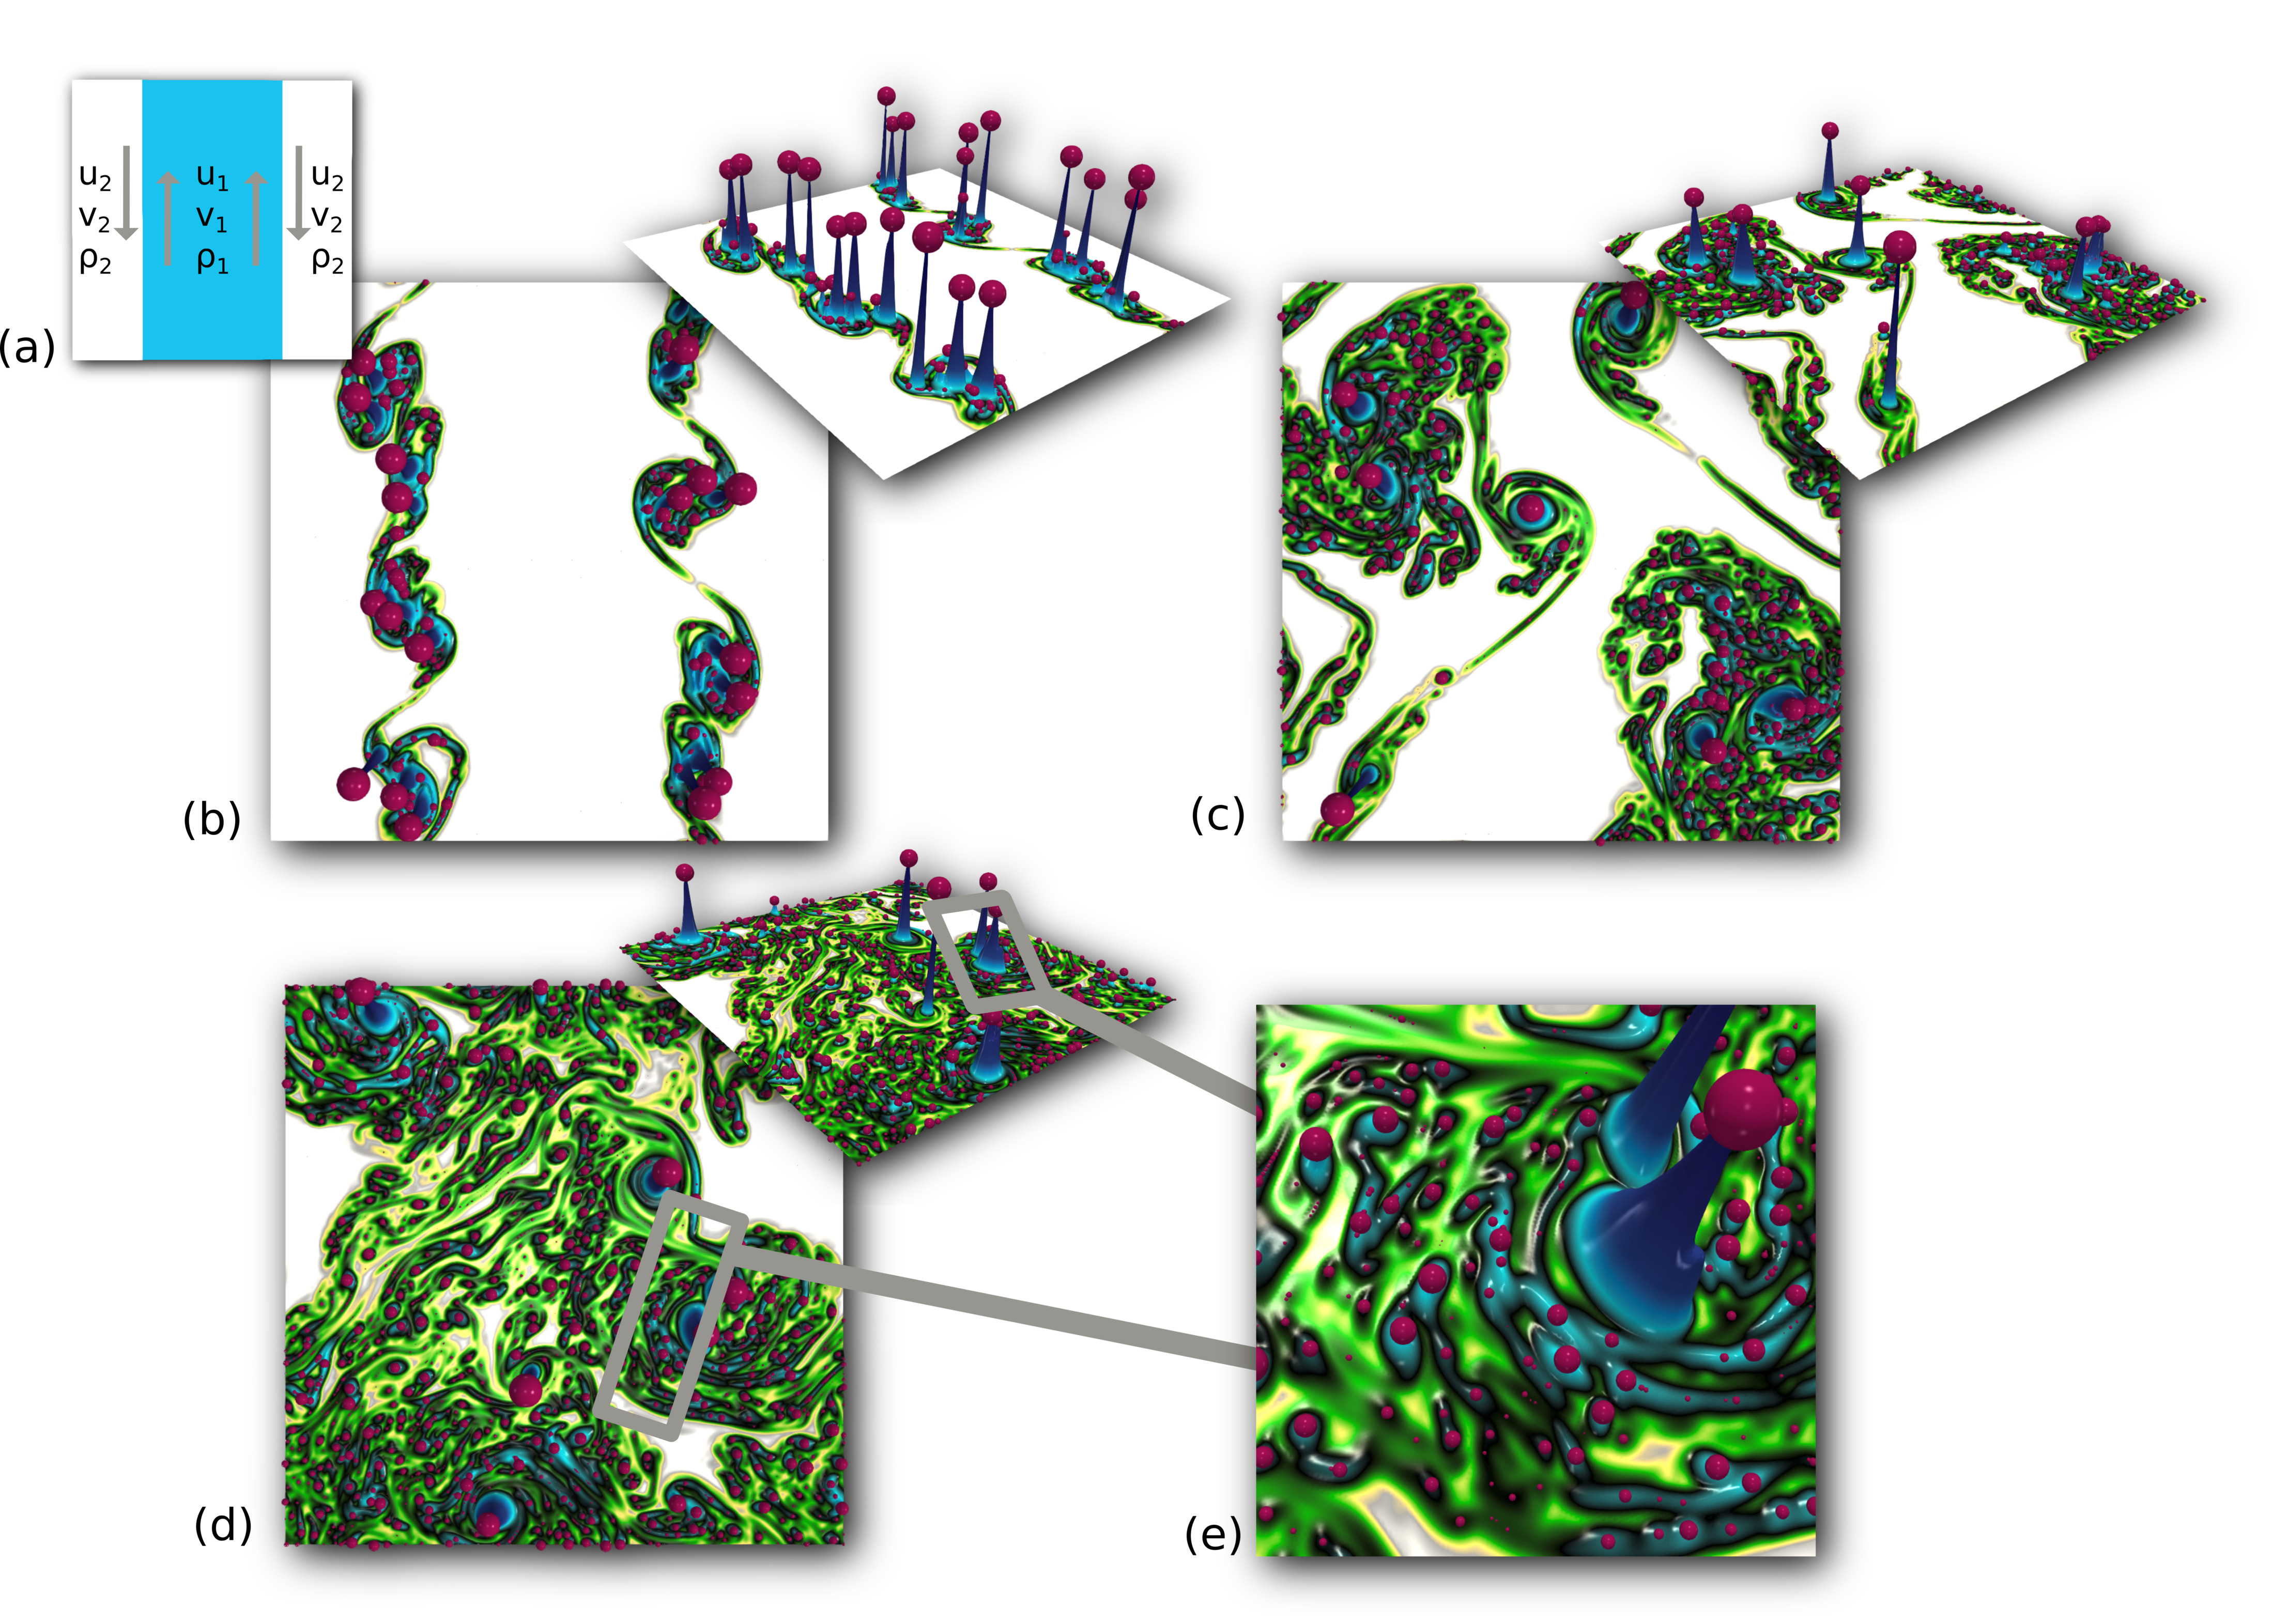
\includegraphics[width=\figureShrink\linewidth]{chapter4_topology_data_analysis/pictures/init_case.jpg}
 \vspace{-2ex}
 \mycaption{Initialization of the Kelvin-Helmholtz instability (a). This simulation was obtained
with the AUSM$^+$-UP solver with a TENO 5 order interpolation at physical times $0.25$(b), 
$0.75$(c) and $1.25$(d). Red spheres scaled by the persistence represent the maximum critical points. Zoom of the turbulence structures (e).}
  \vspace{2ex}
 \label{initcase}
\end{figure}

\subsection{Data description}
The initialization of the KHI was generated with two fluids of different 
densities ($\rho_{1}$, $\rho_{2}$) (\autoref{initcase}a). The
different velocities of opposite direction ($\{u _{1},v_{1}\},\{u _{2},v_{2}\}$) 
of the fluids create a shearing zone where the turbulence appears with the KHI 
(\autoref{initcase}b). While the instability develops over time the main 
vortices grow (\autoref{initcase}c). After a longer simulation time, the main 
structures keep evolving (\autoref{initcase}d) and a large number of 
small-scale vortices appear in the vicinity of large-scale vortices
% around the main structures 
(\autoref{initcase}e) 
leading to a complex turbulent flow. This variation in vortex scale,
% of the
% vortices,
in addition to the chaotic flow geometry,
% of the flow,
is notoriously
challenging for the analysis of turbulent flows.

\begin{table}
\centering
\scalebox{0.8}{
\begin{tabular}{|c|c|c|c|c|c|c|}
\hline
Parameter            & Resolution           & Order                &  Time       
       &  Solver              &  Scheme              &  Total              \\ 
\hline
\hline
                     &                      &                      &             
         &  HLL            &                 &                \\
                     &  256                 &      5               &       t$_0$ 
         &  SLAU2          &  TENO         &                \\
Value                &  512                 &      7               &       t$_1$ 
         &  AUSM$^+$-UP         &  WENO-Z        &                \\
                     &  1024                &                      &       t$_2$ 
         &  Roe            &                &                \\
                     &                      &                      &             
         &  HLLC           &                &                \\                  
                                             
\hline
\hline
Number&3&2&3&5&2&180\\
\hline
\multicolumn{1}{l}{} & \multicolumn{1}{l}{} & \multicolumn{1}{l}{} & 
\multicolumn{1}{l}{} & \multicolumn{1}{l}{} & \multicolumn{1}{l}{} & 
\multicolumn{1}{l}{} 
\end{tabular}
}

\caption{Parameter space of the HYPERION simulation code leading to a total of 180 members for the ensemble dataset used in this study.}
\vspace{-3ex}
\label{tab_parameters}
\end{table}

% This is why, in the section 
% \autoref{sec_experimentalResults} we study how the topological analysis of the 
% % enstrophy can capture features in the KHI and thus help us to compare them. 

The HYPERION simulation code introduced in \autoref{sec_simulation} has been 
used to generate the ensemble dataset. All the simulations have been run on a 
supercomputer 
% of the CEA 
at our institution. Each simulation have been executed in parallel using 16 MPI processes and have been distributed over the supercomputer. The total 
simulation took about 745 CPU hours. The raw data has been dump on disk with the 
metadata stored in XDMF files and the scalar fields in HDF5 files leading to 14 
GB for the entire ensemble dataset. We processed these results to extract the 
enstrophy scalar field (\autoref{eq:enstrophy}) and stored it to a VTK file 
format \cite{Kitware:2003} using an image data structure for regular grids 
(VTI). This reduces the entire ensemble to 600 MB. 

The ensemble dataset corresponds to different computational configurations for 
the same turbulent instability. HYPERION handles different parameter types such 
as scalars or enumerations, which allows the users to compute various numerical 
simulations in the same parametric study. The resolution of the 2D regular grid, 
the simulation time, the interpolation scheme, the order of interpolation and 
the Riemann solvers presented in \autoref{sec_background} are our different 
parameters. \autoref{tab_parameters} details the parameter types and values as 
well as the number of samples per parameter, leading overall to an ensemble of 
$3\times2\times3\times5\times2=180$ members illustrated \autoref{fig_teaser}a. 
Each parameter value of \autoref{tab_parameters} used to run the simulation has 
been stored as meta-data in the VTI files (i.e. \emph{Field Data} in the VTK 
terminology)  to keep track of the computational configuration for later 
analysis down the pipeline.
In order to ease the exploration of the ensemble dataset, we defined a 
SQL-type database using the cinema database feature of TTK \cite{ttk17, ttk19}. 
This representation facilitates the extraction of sub-samples of the ensemble, 
based on standard SQL queries on the simulation parameters 
(\autoref{tab_parameters}).

% This database eases the query to extract sub-samples of the ensemble using the 
% input parameters referenced in \autoref{tab_parameters}.\julien{référencer 
% l'annexe pour le détail technique des temps ?}



\begin{figure}
 \centering
 \vspace{-1ex}
 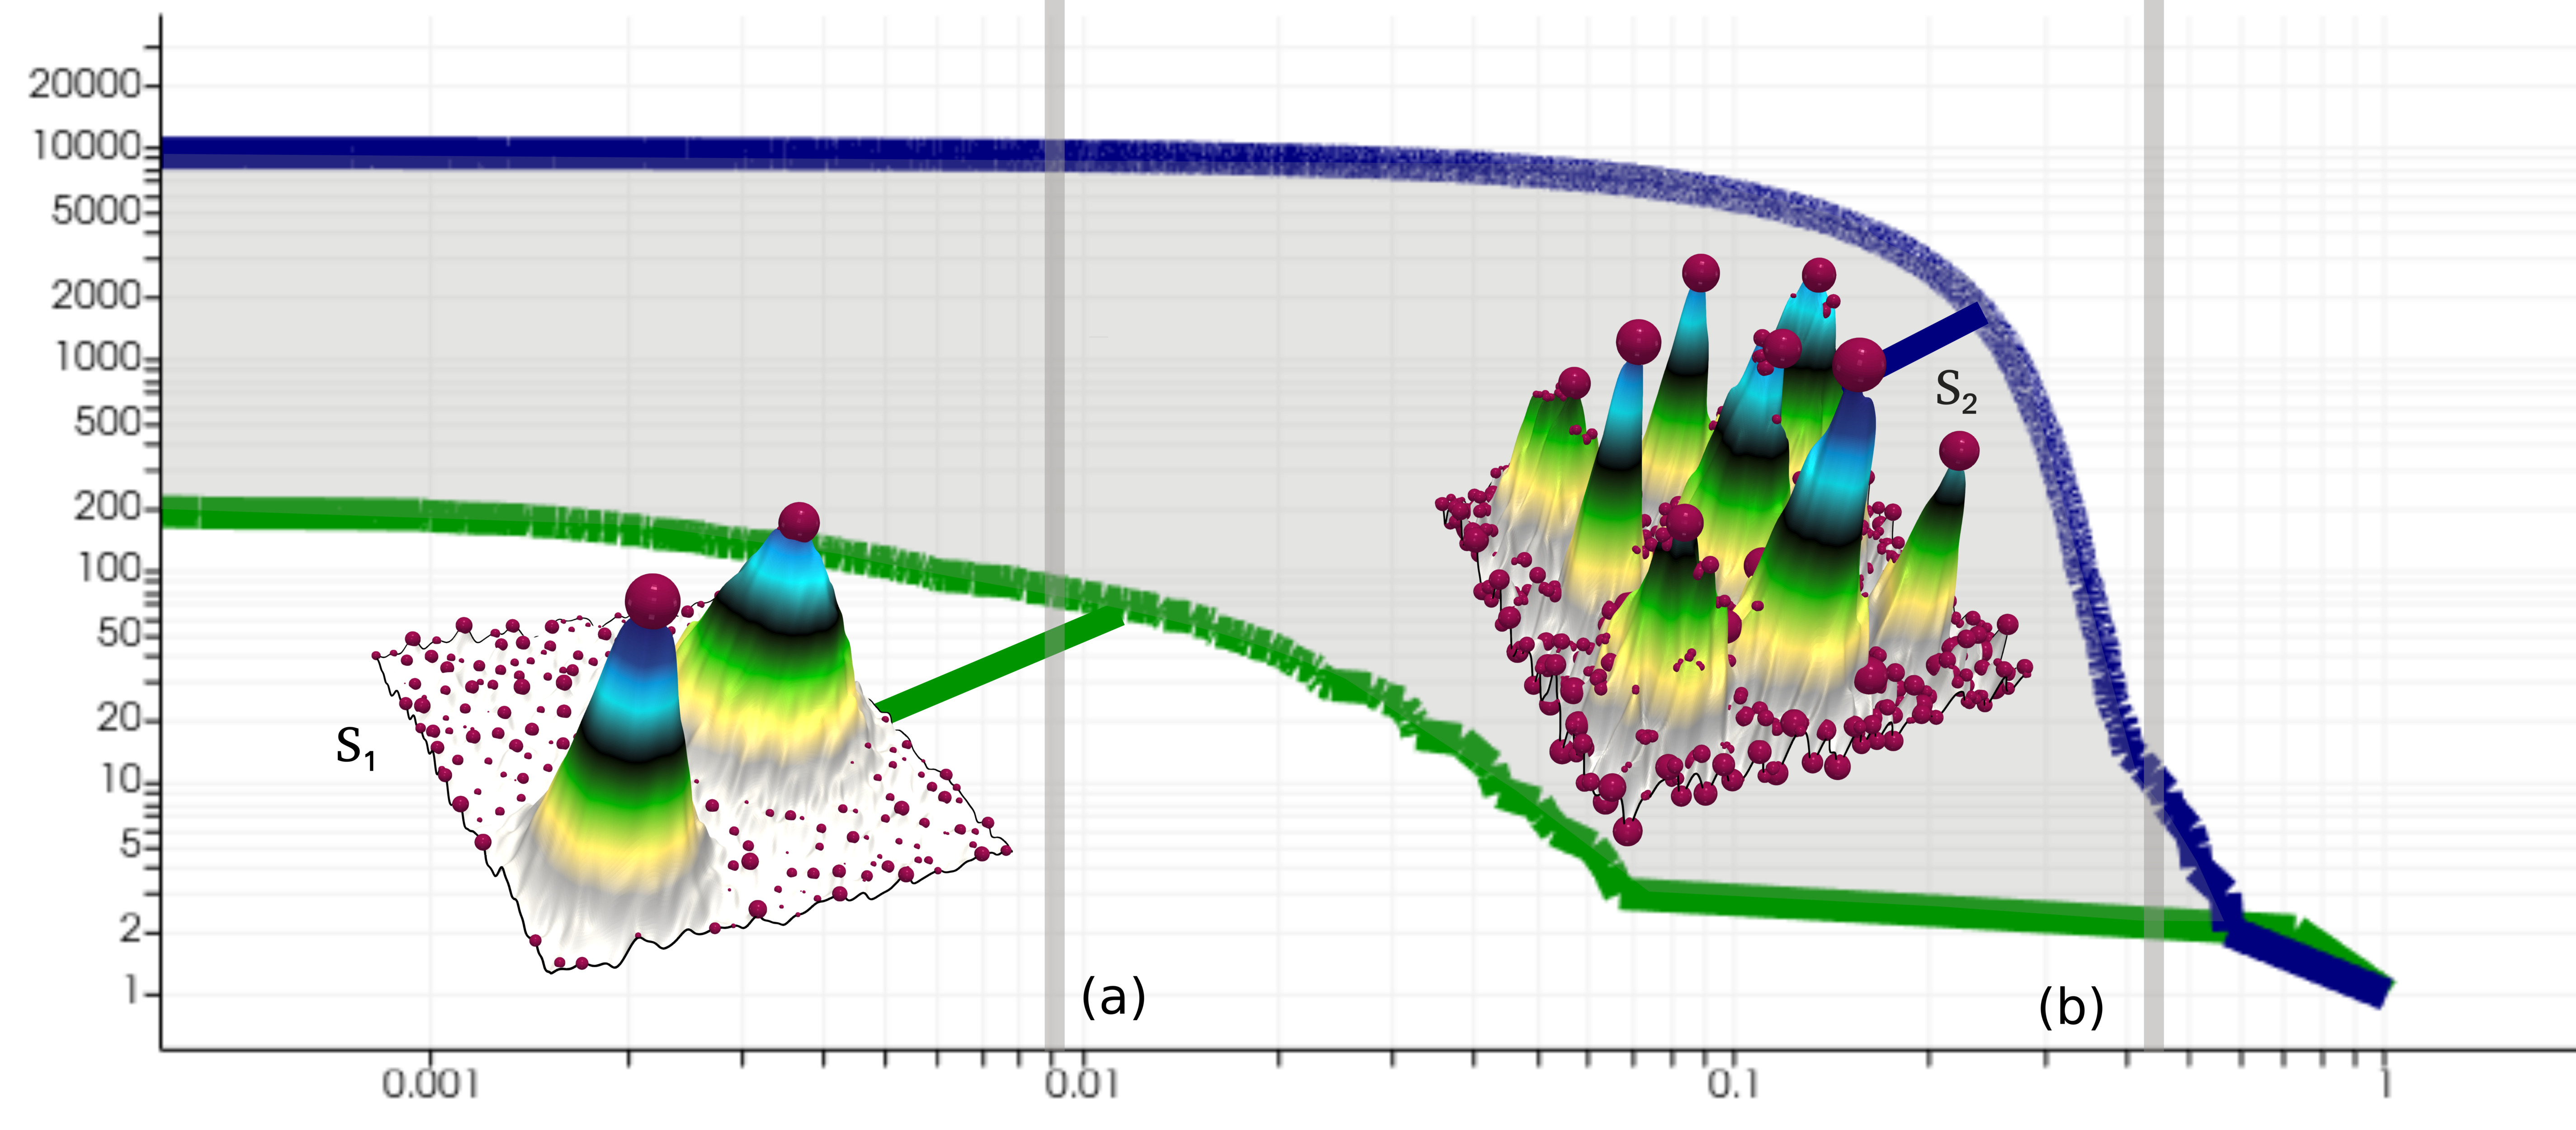
\includegraphics[width=\figureShrink\linewidth]{chapter4_topology_data_analysis/pictures/gaussian_courbe.jpg}
 \mycaption{Persistence curves for two input scalar fields (X-axis: persistence threshold, Y-axis: number of maxima more persistent than X). $S_1$ generated with two Gaussian functions with noise and $S_2$ with 10 Gaussian functions with a stronger noise. Maxima critical points are represented by red spheres scaled by persistence. Vertical line corresponds to
 (a) small persistence critical points, (b) to high persistence. The grey area is the integral difference between the two curves.}
 \label{fig_gaussian_curve}
\end{figure}

\subsection{Problem statement}

% For numerical computation in fluid dynamics there are several methods of interpolation and Riemann solvers.
% For today's engineers who design vehicles it is important to use accurate methods to recover for example heat fluxes, pressure at the walls to be able to dimension correctly their future vehicles.
% Nevertheless, it is also necessary to take into account the calculation time which can be extremely high, especially with 3-dimensional calculations.
% The calculation of the turbulence is then important because this phenomenon will bring fluctuations of the data that we analyze and it is then necessary to capture it with precisions too.
% It is a fractal phenomenon that we analyze by averaging on the domain a value to look at scpectra later.
% With this traditional treatment it is difficult to see a real difference between the numerical methods and especially for the solvers.
% That's why we want to use the topology to maybe guide our choice of numerical methods.
% -- 
Vehicle design, be it in an automotive or aeronautical context, is well known for its high number of constraints that are nowadays most often handled with the help of computational techniques.
In the aeronautical world for instance, engineers today face an incredible challenge wherein they have to be able to predict, at the same time, integral quantities at the wall of the vehicle such as heat flux or pressure as well as three-dimensional phenomena such as flow discontinuities and turbulence.
In other words, engineers have to deal with multiple types of physics and phenomena that have markedly different length- and time-scales but whose interactions are still of great importance to the accuracy of their predictions.
With limited time and resources to conduct the computer-aided simulations, the traditional approach is to rely on numerical strategies that temporally average most of the three-dimensional phenomena and rely more or less on models of turbulence to yield a fast and reasonable forecast.

Even in such a context of approximate simulations, the choice of the ingredients of the numerical recipe matters - methods of reconstruction, Riemann solvers, etc.
Making the right choices can indeed bring a significant increase in fidelity to the engineer, especially in terms of turbulence, by lessening the need for modeling and henceforth bring more margin in the design of the vehicle.
Turbulence is however by nature a chaotic phenomenon and conducting a systematical study of the impact of the different
% aforementioned
numerical ingredients thereupon might prove tricky for a simple reason: beyond a certain level of accuracy, everything will \emph{look} the same.
Detecting the benefits of one method compared to another in that situation will be next to impossible - that is, with traditional techniques.
We propose here to use the ability of topological analysis to discern features that stay otherwise hidden in traditional fluid dynamics postprocessing to help with the choice of the right numerical ingredients. 



\subsection{CFD Hypotheses}
\label{sec_hypotheses}
This section introduces the hypotheses provided by CFD experts, documenting their expectations about ensemble flow variability.
% in the ensemble.}

% \florent{Here are the assumptions considered in this study, provided by CFD experts, with a literature search.}

\label{Hypotheses}
\noindent
\textbf{Hypothesis H1.}
% It is assumed that
TENO induces more turbulence (i.e. more critical points) than
% the
WENO-Z, for all configurations.\\
% no matter the resolution, the time or the solver is.\\
\textbf{Hypothesis H2.}
Order 5 and 7 are equivalent for Kelvin Helmholtz instabilities.\\
% In the literature, studies have been conducted on turbulence and notably on Kelvin Helmholtz to show that orders 5 and 7 are equivalent. We therefore try to find an independence of the orders using our topological analysis.\\
\textbf{Hypothesis H3.}
The HLL solver should provide a significantly distinct description, for all configurations.\\
% It is assumed that the HLL solver describes very differently the instabilities for all resolutions and schemes. It's a dissipative solver and doesn't take into account the dissipative
% contact discontinuities.\\
\textbf{Hypothesis H4.}
The HLLC and Roe solvers should provide equivalent outputs for all configurations.\\
% (and should therefore belong to the same cluster).\\
% It is assumed that HLLC and Roe are in the same cluster for all resolutions and schemes. These solvers are of FDS type, they take into account the contact discontinuities, but do not adapt to all Mach.\\
\textbf{Hypothesis H5.}
The
% It is assumed that
SLAU2 and AUSM$^+$-UP solvers should provide equivalent outputs for all configurations.\\
% are in the same cluster for all resolutions and schemes.
% They are FTS type solvers, they have the characteristics of being not very dissipative and they adapt to all speeds.\\

The above hypotheses are direct consequences of
% prior experimental
observations, or
% solver
design choices. For instance, the TENO scheme has been reported to capture turbulence more accurately \cite{peng2021efficient}, which is expressed by Hypothesis H1. Similar kinetic energy curves (\autoref{energie}) have been reported for the orders 5 and 7, which is expressed by Hypothesis H2. The HLL solver, which is a dissipative approach, is known to model contact discontinuities poorly in contrast to more recent solvers, which is expressed in Hypothesis H3 \cite{toro2013riemann}. Finally, unlike the SLAU2 and AUSMUP (FTS type) solvers, the HLLC and RoE (FDS type) solvers have been reported to provide unphysical results at both low and high velocities (resulting in local oscillations in pressure and density), which is expressed in Hypotheses H4 and H5. %\cite{qu2021review}.

From a practical point of view, the validation of these hypotheses has a major impact for the engineers when setting up their simulations. For instance, the validation of the Hypothesis H1 would justify the usage of a more computationally expensive scheme (TENO), while the validation of the Hypothesis H2 would enable the usage of less computationally expensive orders (5 instead of 7). Finally, the validation of the Hypotheses H3, H4, and H5 would help engineers properly select the most appropriate solvers, based on their flow characteristics.
% expected velocities.
Then, overall, the validation of these hypotheses
% is important towards the
would provide reliable rules-of-thumb for the tuning of the solvers,
% enables more confidence when
% proper
% tuning of the solvers,
to achieve the best balance between accuracy and speed.

% \florent{Referring to the publication of liu fu,(Add ref \cite{peng2021efficient}) who developed the TENO scheme, and who compared it to the weno scheme on several test cases, the TENO has the ability to capture with more accuracy the turbulence phenomenon.  By looking at the topological approaches to the results obtained between these two schemes we should observe differences in the number of structures that are reconstructed(H1).}
% \florent{A study on weno(ref) schemes, using a KHI as a test case, shows that for order 5 and 7, a similar result is obtained on the kinetic energy curves (\autoref{energie}).}
% \florent{Assumptions H4 and H5 allow us to compare Riemann solvers that do or do not calculate all velocities in a numerical simulation. According to the literature (add ref). The HLLC and ROE solvers fail to calculate both high and low velocities, which leads to small oscillations (pressure or density) in the simulation results, unlike the SLAU2 and AUSMUP solvers.
% Validating the Hypotheses will help engineers to choose which tools to use to set up their numerical simulations by minimising the computational cost and to gain precision in the numerical methods used.}




\subsection{Baseline analysis}
Traditional approaches for turbulent data analysis (\autoref{energie}) are based on an average of
quantities of interest, such as flow energy (\autoref{sec_relatedWork}).
The $L_2$ norm is another established distance for comparing scalar fields. Both strategies bear similarities in their averaging artifacts: they cannot distinguish the contribution
of small structures from the global flow, because these are masked by the weight
of larger vortices.
%
% However, this average strategy
% % the energy or the enstrophy (see
% % \autoref{sec_relatedWork} and \autoref{energie}).
% such an averaging is similar to the averaging
% effect of the $L_2$-norm, when used for comparing enstrophy fields.
% % These averages correspond to the calculation of $L_2$-distances between the
% % solutions.
% In particular, this distance does not allow to see the contribution
% of the small structures to the global flow because they are masked by the weight
% of larger structures.
Moreover, the $L_2$-norm is also very sensitive to mild geometric variations,
whereas the chaotic nature of turbulent flows induces major geometric
variations between ensemble members.
This motivates the usage of  topological methods to capture
features in the KHI that will help us compare the members
(\autoref{sec_experimentalResults}). In the remainder, we will systematically compare our protocols based on topological distances (\autoref{sec_protocols}) to the $L_2$ norm, considered as the baseline approach, and detailed comparisons will be provided (\autoref{sec_experimentalResults}).
